\newcommand\UniversiteAdi{Niğde Ömer Halisdemir Üniversitesi}
\newcommand\BolumAdi{MEKATRONİK BÖLÜMÜ}
\newcommand\DersKodu{MKT2002}
\newcommand\DersAdi{BİLGİSAYARLI KONTROL SİSTEMLERİ}
\newcommand\SinavAdi{Ödev 2}
\newcommand\SinavTarihi{10.03.2025}
\newcommand\SinavSaati{10:00}
\newcommand\SinavSuresi{90dk}

\pagestyle{fancy}
\fancyhf{} % clear existing header/footer entries
\fancyhead[R]{Öğrenci No:\hspace{4.5cm}}
\fancyhead[L]{Ad Soyad:\hspace{7cm}}
\noindent
\begin{tabular}{
    p{0.15\linewidth}
    p{0.15\linewidth}
    p{0.3\linewidth}
    p{0.1\linewidth}
    p{0.15\linewidth}}
    \multicolumn{5}{c}{\textbf{\BolumAdi}}\\
    \multicolumn{5}{c}{\textbf{\DersAdi}}\\\hline
    \multicolumn{1}{|r|}{Ders Kodu:}&
    \multicolumn{1}{|c|}{\DersKodu}&
    \multicolumn{1}{|c|}{}& 
    \multicolumn{1}{|r|}{Tarih:}&
    \multicolumn{1}{|c|}{\SinavTarihi} \\\hline
    \multicolumn{1}{|r|}{Sınav Türü:}&
    \multicolumn{1}{|c|}{\SinavAdi}&  
    \multicolumn{1}{|c|}{}&
    \multicolumn{1}{|r|}{Saat:}&
    \multicolumn{1}{|c|}{\SinavSaati}\\\hline
    \multicolumn{1}{|r|}{Dönemi:}&
    \multicolumn{1}{|c|}{2024-2025}&
    \multicolumn{1}{|c|}{}&
    \multicolumn{1}{|r|}{Süre:}&
    \multicolumn{1}{|c|}{\SinavSuresi} \\\hline
    &&&&\\
\end{tabular}\\\\
\noindent\begin{center}
\begin{tabular}{|r|c|}\hline
    &\textbf{Toplam}\\\hline
    \textbf{Puan:} &\textbf{100}\\\hline
    \textbf{Not:}  &100\\\hline
\end{tabular}\end{center}
\noindent\textbf{Uyarı:}
\begin{itemize}\bfseries
    \item Soruları dikkatlice okuyunuz. Hesap makinesi kullanılabilir.
    \item İşlemleri atlamadan ve ayrıntılı olarak veriniz. Sadece nümerik yanıtlar veya çizimler ara işlemler olmadan kabul edilmemektedir.
\end{itemize}
\noindent\textbf{Soru:}  S tanım bölgesinden z tanım bölgesine geçiş 
\begin{equation}
    z=e^{sT}
\end{equation}
ile yapılmaktadır. $s=-1\pm 1i$ olarak verilen kutup çifti için $T$'nin değişimi ile z tanım bölgesinde kutup çiftinin hareketini nümerik yöntemlerle belirleyiniz ve bir grafik olarak gösteriniz. 

Örnekleme zamanına göre değişim Şekil~\ref{fig:plot1} ile gösterilmiştir. Burada $T\rightarrow 0$ seçilmesi durumunda $e^{sT}\rightarrow 1$ ve $T\rightarrow \infty$ seçilmesi durumunda ise $e^{sT}=e^{-\infty}\rightarrow 0$ elde edilecektir. Dolayısıyla birim çember üzerinde başlayıp merkeze doğru bir hareket elde edilmektedir.  
\begin{figure}[!htb]
    \centering
    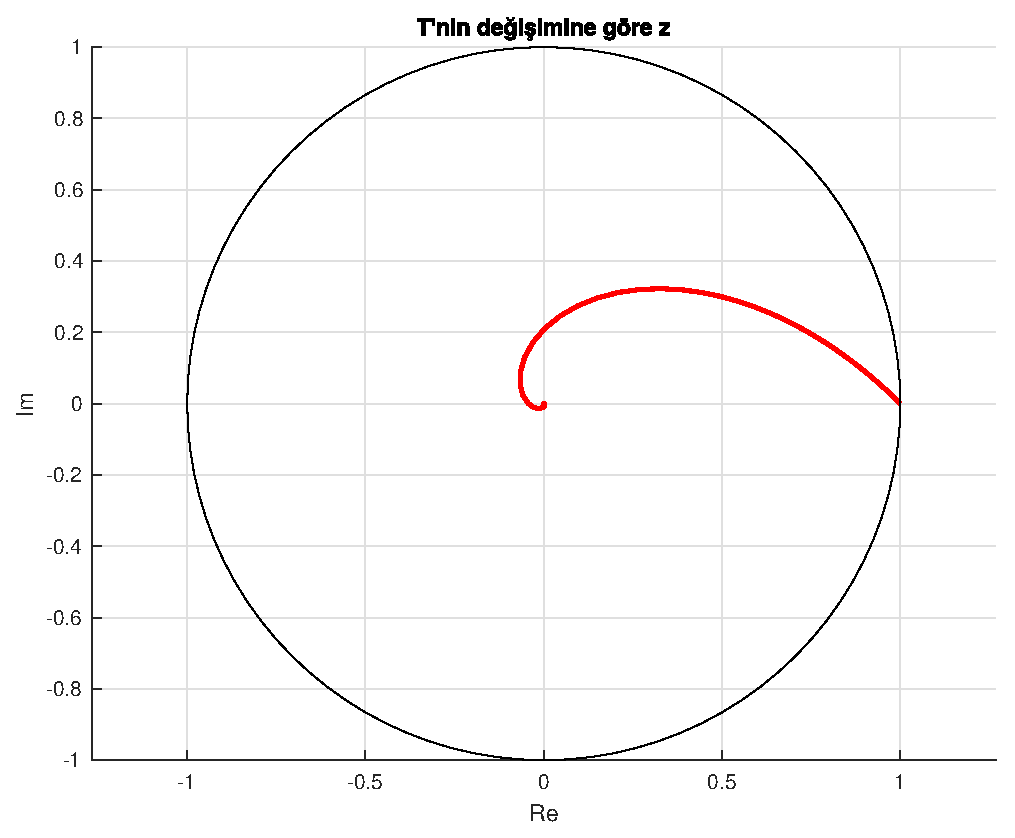
\includegraphics[width=0.5\textwidth]{plot1}
    \caption{Örnekleme zamanına göre z tanım bölgesinde kutbun hareketi}\label{fig:plot1}
\end{figure}